% !TEX TS-program = pdflatex
% !TEX root = ../ArsClassica.tex

%************************************************
\begin{appendices}
%************************************************
\chapter{CPLEX}
ILOG CPLEX is a tool for solving different types of problems. One of those category are the Linear Programming (LP) problems, of the form:
\[
Maximize \ (or \ minimize): \quad \quad c_1 x_1 + c_2 x_2 + c_n x_n 
\]
\[
Subject \ to: \quad \quad a_{11} x_1 + a_{12} x_2 + ... + a_{1n} x_n \sim b_1 
\]
\[
\qquad \qquad \qquad \quad \ a_{21} x_1 + a_{22} x_2 + ... + a_{2n} x_n \sim b_2
\]
\[
\qquad \qquad \qquad \quad \ ...
\]
\[
\qquad \qquad \qquad \quad \ a_{m1} x_1 + a_{m2} x_2 + ... + a_{mn} x_n \sim b_m
\]
\[
With \ these \ bounds: \qquad \qquad l_1 \leq x_1 \leq u_1
\]
\[
\qquad \qquad \qquad \qquad \ \ \  ...
\]
\[
\qquad \qquad \qquad \qquad \qquad \qquad \qquad l_n \leq x_n \leq u_n
\]
Where $\sim$ can be $\leq$, $\geq$ or $=$, and the upper bounds $u_i$ and lower bounds $l_i$ may be positive infinity, negative infinity, or any real number. In the mixed integer case some of the variables are required to only assume integer values.\\
In particular, we have used the \textsc{CPLEX} Callable Library, which is a C library, that allows the programmer to embed \textsc{CPLEX} optimizers in application written in C. Thus, we have used \textsc{CPLEX} as a tool for solving Mixed Integer Programming problems suche as Wind Farm Cable Problem instances.\\
In this appendix we want describe the main method that we use to create the \textsc{CPLEX} environment, to instantiate a problem to populate a problem object.

\section{Initialization of \textsc{CPLEX} Environment}
The first thing to do in an application that uses \textsc{CPLEX} is create a \textsc{CPLEX} environment:
\begin{itemize}
\item \textit{CPXENVptr env = CPXopenCPLEX(\&error)}: initializes a \textsc{CPLEX} environment and returns a pointer to it; the parameter is a pointer to an integer where an error code is placed by the routine.
\end{itemize}

Then a \textsc{CPLEX} problem object must be created:
\begin{itemize}
\item \textit{CPXLPptr lp = CPXcreateprob(env, \&error, "Name of problem")}: this method returns a pointer to the \textsc{CPLEX} problem object. The problem that is created is an LP minimization problem with zero constraints, zero variables and an empty constraint matrix.
\end{itemize}

\section{Population of a problem}
Now we have initialize the environment and we must set the objective function and the constraints of our model.
To add a variable in the our objective function we must use:
\begin{itemize}
\item \textit{CPXnewcols(env, lp, ccnt, \&obj, \&zero, \&ub, \&type, cname)}: adds ccnt empty columns to the specified \textsc{CPLEX} problem object lp. For each column, we must specify the objective coefficient, the lower and upper bounds, the variable type and the name of the variable.
\end{itemize}

Then we have to add the constraints:
\begin{itemize}
\item \textit{CPXnewrows(env, lp, rcnt, \&rhs, \&sense, NULL, cname)}: adds rcnt empty constraints to a specified \textsc{CPLEX} problem object lp; for each row, we specify the right hand side value, sense, range value (NULL), and name of the constraint; the constraint coefficients in the new rows are zero.
\end{itemize}

To set the coefficients of the constraints in a row we use:
\begin{itemize}
\item \textit{CPXchgcoef (env, lp, row, column, coeff)}: changes a single coefficient in the constraint matrix in the position specified by (row, column).
\end{itemize}

\section{\textsc{CPLEX} execution and setting \textsc{CPLEX} parameters}
Now we must to start the execution of \textsc{CPLEX} and get the result.\\
Before the \textsc{CPLEX} starts we can set some parameters relative to its execution:
\begin{itemize}
\item \textit{CPXsetTYPEparam(env, CPX\_PARAM\_XXX, value)}: this function depends by the type of parameter, its type must substitute TYPE in the invoketion; the parameter that will be setted  is the second parameters of the function. The last is the starting value.
\end{itemize}

Now we can execute the \textsc{CPLEX} solver to solve our problem:
\begin{itemize}
\item \textit{CPXmipopt(env,lp)}: finds a solution to the problem lp.
\end{itemize}
Then get the informations about the solution with:
\begin{itemize}
\item \textit{CPXgetobjval(env, lp, \&sol\_value)}: writes in \textit{sol\_value} the solution objective value.
\item \textit{CPXgetx(env, lp, sol , 0, ncols-1)}: writes in \textit{sol} the solution variables values.
\end{itemize}

Before the end of execution we must free the space occupied by the problem with:
\begin{itemize}
\item \textit{CPXfreeprob(env, \&lp)}: that free the space occupied by the lp.
\item \textit{CPXcloseCPLEX(\&env)}: that release the pointer relative to the \textsc{CPLEX} environment.
\end{itemize}


\chapter{Shell script}
The collection of the results is an important part of our software development. It gives us the possibility to run the same code on different instances, to collect the results in a accessible way, to compare results obtained with different CPLEX parameters and finally gives us the convenience to store all the results of a run in the same folder. 
For those reasons, when we were still at the beginning of the development we create a \textit{shell script} that automate the process. It is composed by some parts:
\begin{enumerate}
\item Make: compiles the code at the actual state.
\item Creates the plot folder and the results folder named with the actual timestamp.
\item Defines the the command line parameter in the \textit{settings} variable.
\item Starts a cycle iterating over all the .turb files in the data folder, that contains all the instances. For each iteration it executes the wfcp script and saves the logs in the right folder giving them a name that associate it to the instance. The \textit{cSub} variable is set in order to use the correct $C$ for each instance.
\item Sorts some files, also the .png results if present.
\item Creates the settings.txt file with the execution settings of that run.
\item Creates the results.csv file that collects all the results coming from the logs.
\end{enumerate}

The script automatically detects the working directory from which the script is launched, so it is adaptable to different environments if the folder structure is the following:
\begin{itemize}
\item main directory
\item data: contains all the .turb and .cbl file
\item runs: contains the results 
\item src: contains the script files and the multi\_wfcp.sh file. 
\end{itemize}

Here the code of the \textit{multi\_wfcp.sh} file:
\newpage
\lstinputlisting[language=bash,caption={Shell multi\_wfcp.sh script}]{/home/davide/dev/WFCP/src/multi_wfcp.sh}

\chapter{Input string parameters}
In our code we tried to parameterize all the compilation options, in order to avoid to change the code for little changes or different tests. \\
Here we describe all the parameter in a ready-to-use list of options: 
\begin{itemize}
\setlength{\parskip}{0pt}
\setlength{\itemsep}{0.5pt plus 1pt}
\item \textbf{fc} : input cables file
\item \textbf{ft} : input turbines file
\item \textbf{C} : capacity of root
\item \textbf{time\_loop} : time for loop in loop/heuristic method
\item \textbf{time\_limit} : total time limit
\item \textbf{time\_start} : time start to heuristic method
\item \textbf{model} : model type
\begin{enumerate}\setcounter{enumi}{-1}
\setlength{\parskip}{0pt}
\setlength{\itemsep}{0pt plus 1pt}
	\item \textsc{CPLEX} model
	\item Matrix model
\end{enumerate}
\item \textbf{rins} : rins
\item \textbf{relax} : relax
\begin{enumerate}\setcounter{enumi}{0}
\setlength{\parskip}{0pt}
\setlength{\itemsep}{0pt plus 1pt}
	\item relax on station capacity
	\item relax on flow
	\item relax on flow + out edges
	\item[] else : no relax
\end{enumerate}
\item \textbf{polishing\_time} : polishing time
\item \textbf{gap} : gap to terminate
\item \textbf{seed} : random seed
\item \textbf{threads} : n threads
\item \textbf{CC} : Computational Context
\begin{enumerate}\setcounter{enumi}{-1}
\setlength{\parskip}{0pt}
\setlength{\itemsep}{0pt plus 1pt}
	\item Normal execution with no cross cable as normal constraints
	\item Lazy constraints to the model
	\item Loop Method
	\item Normal execution + lazy callback
	\item Hard Fixing
	\item Soft Fixing
	\item Heuristic
	\item Heuristic Loop to have multiple solution
	\item Heuristic with 1-opt
	\item Tabu Search
	\item Multi-start
	\item[] else: Normal Execution
\end{enumerate}
\item \textbf{soft\_fix} : Type of soft fixing
\begin{enumerate}\setcounter{enumi}{0}
\setlength{\parskip}{0pt}
\setlength{\itemsep}{0pt plus 1pt}
	\item Asimmetric Local Branching
	\item Simmetric Local Branching
	\item Asimmetric RINS
	\item Simmetric RINS
\end{enumerate}
\item \textbf{hard\_fix} : Type of hard fixing
\begin{enumerate}\setcounter{enumi}{0}
\setlength{\parskip}{0pt}
\setlength{\itemsep}{0pt plus 1pt}
	\item Random hard fixing
	\item RINS
\end{enumerate}
\item \textbf{times} : times to do heuristic
\item \textbf{names} : 1 for more clear file names
\end{itemize}

\chapter{GNU PLOT}
Gnuplot is the command-line program, which can generate two and three dimensional plots of functions, data and data fits, that we have used to plot the solutions of the Wind Cable Farm problem instances.\\
To plot a solution we created the following script to be used by gnuplot to plot the data.\\
\begin{lstlisting}[language=bash,caption={Gnuplot script}]
set autoscale
set term wxt title 'cost of solution'
plot \
	'plot/plot_datastd_#cable1.dat' using 1:2 with lines lc rgb "#color1" lw 2 title "Cable 1",\
	'plot/plot_datastd_#cable1.dat' using 1:2:(0.6) with circles fill solid lc rgb "black" notitle,\
	'plot/plot_datastd_#cable1.dat' using 1:2:3     with labels tc rgb "black" offset (0,0) font 'Arial Bold' notitle
replot \
	'plot/plot_datastd_#cable2.dat' using 1:2 with lines lc rgb "#color2" lw 2 title "Cable 2",\
	'plot/plot_datastd_#cable2.dat' using 1:2:(0.6) with circles fill solid lc rgb "black" notitle,\
	'plot/plot_datastd_#cable2.dat' using 1:2:3     with labels tc rgb "black" offset (0,0) font 'Arial Bold' notitle
.
.
.
replot \
	'plot/plot_datastd_#cable3.dat' using 1:2 with lines lc rgb "#color3" lw 2 title "Cable 3",\
	'plot/plot_datastd_#cable3.dat' using 1:2:(0.6) with circles fill solid lc rgb "black" notitle,\
	'plot/plot_datastd_#cable3.dat' using 1:2:3     with labels tc rgb "black" offset (0,0) font 'Arial Bold' notitle

\end{lstlisting}
With \textit{\#cableX} that depends by the solution and the \textit{\#colorX } is obtained from an array that contains twenty colors, this is made to have different colors for different cables.\\
The data file \#cableX.dat contains pair of nodes that will be linked with the cable X, also this file is created at run time. This files, for any cables, are like:
\newpage
\begin{lstlisting}[language=bash,caption={Data file containing cables}]
node1.x	node1.y
node2.x	node2.y

node3.x	node3.y
node4.x	node4.y
.
.
.
node(n-1).x	node(n-1).y
node(n).x		node(n).y
EOF
\end{lstlisting}
Once that the files are created (one for the script and K for the cables, where K equals to the number of cables used in the solution), we manage the execution of the script by the pipe with three command:
\begin{lstlisting}[language=bash,caption={Script execution}]
FILE *gp = popen("gnuplot -p", "w");  // open gnu plot on the pipe 
fprintf(gp, "load 'plot/script_plot.p'\n"); // run the script and show the plot
fclose(gp); // close the plot
\end{lstlisting}
Figure \ref{img:plotExample} shows a plot example. 
\begin{center}
	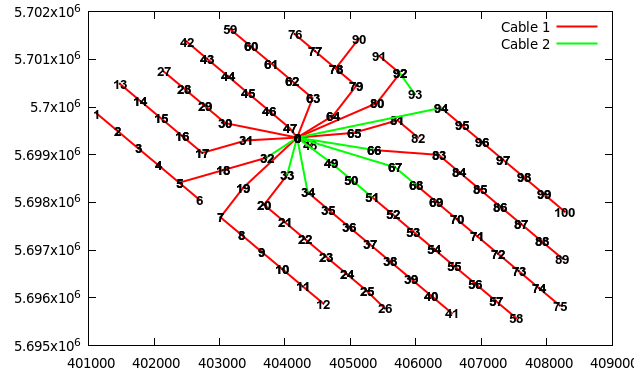
\includegraphics[scale=0.5]{Graphics/plot.png}
	\captionof{figure}{Plot example using gnuplot}
	\label{img:plotExample}
\end{center}



\chapter{Performance Profile}
The performance profile,proposed by Elizabeth D. Dolan and Jorge J. Moré in 2002 [\cite{dolan2002benchmarking}], is a tool to evaluate and compare the performance of the set of solvers S on a test set P. This tool, given a set of benchmarks, returns, as seen, a plot with an evaluation function for each method used.\\
The benchmarks are represented as a table, where each row represents the results obtained from each methods for the same instance.
The X axis measures the percentage of wins with respect to the other methods on the metric we choose as wins (objective function, execution time). The Y axis represents the time ratio and for each different value of it the tool measures the new percentage of wins if the best result obtained in each instance were multiplied for that time ratio.\\
In practice, this tool allow us to evaluate the methods depending on how many times they win and, when that does not happen, in base on how far they are from the best one. In this way we can choose the methods that on average get better results.

\chapter{Performance Variability and Random Seed}
The performance of MIP solvers is subject to some variability that appears when changing from different computing platforms. The literature case [\cite{danna2008performance}], shows us that it could happen that the same instance, with the same code is solved at the root node in one platform, and requires 1426 nodes in another. It is even possible to have different results even if we’re comparing two runs in different partition of the same machine. According to [\cite{lodi2013performance}] also the permutation of rows and/or columns of a model could lead to different performance. The performance variability is common for all the different MIP solvers. 
The reason of that, in a simplified view, is that the small differences of precision between different environment can lead to different branching variables. Infact the Branch and Bound approach can be viewed as a “chaotic” dynamic system because little variations lead to big changes. \\
In literature there are some approaches to this problem and also exploiting this situation for a better overall solver performance: developing pseudo-cost formulas that selects the branching variables in a more robust way or to try some different parameter tuning and evaluate which is the best alternative (this solution adds a computational overhead). \\
Also, CPLEX offers a possible solution giving the random seed parameter that can be used to change the initialization of the random number generator that is used in some internal operations. The random seed triggers random variability, giving the possibility to collect statistics of different runs for more reliable results. \\
For the purpose of our research, the performance variability is not a central question, however it is important for two reasons. First, to understand that the same code applied to the same instance can lead to different solutions depending on the environment. Second, because a variability means that it is possible to take different choices, that means there’s a way to choose (a posteriori) the best option and improve again the performance. 



%************************************************
\end{appendices}



